% Trust by Replay: Hash-Verified Simulation Results for Model Context Protocol Tool Use
% Target: USENIX Security Symposium 2026
% Template: usenix2019_v3.sty (USENIX Security format)
% Status: Complete draft — all sections written
% Paper ID: P1-MCP (MCP tool-use trust layer in Program 1: Trust-by-Construction)

\documentclass[letterpaper,twocolumn,10pt]{article}
% Local sanity compile: if vendor sty is absent (download from usenix.org templates),
% fall back to plain article. Camera-ready builds use the real sty on USENIX infra.
\IfFileExists{usenix2019_v3.sty}{\usepackage{usenix2019_v3}}{\typeout{Skipping usenix2019_v3: vendor sty absent; local compile uses default article class.}}

% Standard packages
\usepackage{amsmath,amssymb}
\usepackage{graphicx}
\usepackage{booktabs}
\usepackage{xcolor}
\usepackage{listings}
\usepackage{hyperref}
\usepackage{balance}
\usepackage{enumitem}
\usepackage{subcaption}
\usepackage{tikz}
\usetikzlibrary{arrows.meta,positioning,shapes.geometric,fit,calc}

% Draft-mode annotations
\newcommand{\todo}[1]{\textcolor{red}{\textbf{[TODO: #1]}}}

% Listing style for TypeScript / JSON
\lstdefinelanguage{TypeScript}{
  keywords={interface, readonly, void, null, string, number, boolean, Record, unknown, Promise, export, const, let, function, return, if, for, type, class, new, async, await, throw, extends, implements},
  keywordstyle=\bfseries\color{blue!70!black},
  commentstyle=\itshape\color{green!50!black},
  stringstyle=\color{orange!70!black},
  morecomment=[l]{//},
  morecomment=[s]{/*}{*/},
  morestring=[b]',
  morestring=[b]",
  morestring=[b]`,
}
\lstset{
  basicstyle=\scriptsize\ttfamily,
  breaklines=true,
  frame=single,
  language=TypeScript,
  numbers=left,
  numberstyle=\tiny\color{gray},
  xleftmargin=1.5em,
  aboveskip=0.5em,
  belowskip=0.5em,
}

% Convenience
\newcommand{\cael}{\textsc{Cael}}
\newcommand{\mcp}{\textsc{Mcp}}
\newcommand{\holoscript}{HoloScript}

% Lotus petal data contract — \measuredFrom{<artifact>} marks values that come
% from a runnable artifact in the repo. Renders nothing in the PDF; grep target
% for scripts/build-lotus.mjs (research/2026-04-26_lotus-petal-data-contract.md §3+§4).
\providecommand{\measuredFrom}[1]{}

\begin{document}

\title{\Large \bf Trust by Replay: Hash-Verified Simulation Results\\for Model Context Protocol Tool Use}

\author{
{\rm Joseph Krzywoszyja}\\
Independent Researcher\\
\texttt{brianonbased@gmail.com}
}

\maketitle

% ═══════════════════════════════════════════════════════════════════════════
% ABSTRACT
% ═══════════════════════════════════════════════════════════════════════════

\begin{abstract}
Large language model (LLM) agents increasingly invoke external tools via the
Model Context Protocol (MCP) to perform computations they cannot execute
natively---structural simulations, thermal analysis, fluid dynamics. The MCP
specification explicitly states that tool annotations are ``considered
untrusted,'' yet provides no mechanism for the agent to verify that a tool's
results are correct. Recent work demonstrates that MCP tools can embed
covertly malicious logic while returning plausible results (tool poisoning),
and the current mitigation---human approval per tool call---does not scale.

We present \emph{Trust by Replay}, the first system that attaches
cryptographic provenance to MCP simulation tool responses. When an LLM calls
a simulation tool (e.g., \texttt{solve\_structural}), the server executes the
computation inside a \emph{contracted sandbox} that enforces six formal
guarantees (geometry integrity, unit validation, deterministic stepping,
interaction provenance, auto-provenance, and replay). A \emph{Causal
Agent-Environment Loop} (\cael{}) hash chain records every simulation step,
interaction, and state transition as a JSONL trace. The tool response includes
both the result and the complete trace; a verifier---the LLM itself, a
separate agent, or a third-party auditor---can independently replay the trace
and detect any tampering via hash-chain breakage.

We implement Trust by Replay in a production MCP server (233 tools as of 2026-04-20 --- see \texttt{docs/NUMBERS.md}; TypeScript,
WebGPU-accelerated solvers) and evaluate it on structural and thermal
simulation workloads. At $N{=}500$ timed iterations, contract enforcement
does not exhibit a stable positive overhead fraction relative to TET4 solver
wall-clock time; medians track V8/GC scheduling noise rather than a dominant
additive cost. Trace size scales linearly with simulation steps at
$\sim$180 bytes per entry. Hash-chain verification runs in $O(n)$ time with
zero false positives and zero false negatives on our test suite. Full
simulation replay, the strongest verification mode, requires compute
proportional to the original execution but catches result-substitution attacks
that hash-only verification cannot. To our knowledge, this is the first
constructive solution to the tool result verification problem identified in
the MCP specification.
\end{abstract}

% ═══════════════════════════════════════════════════════════════════════════
% 1. INTRODUCTION
% ═══════════════════════════════════════════════════════════════════════════

\section{Introduction}
\label{sec:intro}

The Model Context Protocol (MCP)~\cite{mcp-spec} has emerged as the dominant
standard for connecting large language models to external tools. Originally
introduced by Anthropic in November 2024 and transferred to the Linux
Foundation's AI \& Data division in March 2025, MCP defines a JSON-RPC
interface through which LLM agents discover, invoke, and receive results from
tools hosted on local or remote servers. As of mid-2026, MCP is supported by
every major LLM provider and integrated into dozens of agent frameworks.

The protocol's design, however, embeds a fundamental trust asymmetry. The MCP
specification states:

\begin{quote}
\emph{``Tool annotations are primarily informational and are not
  considered trusted. Clients SHOULD NOT make security-critical decisions
  based solely on tool annotations.''}~\cite{mcp-spec}
\end{quote}

\noindent This warning is well-founded. Hou et al.~\cite{hou2025mcp}
demonstrate that MCP tools can embed covertly malicious logic---altering file
paths, exfiltrating data, or returning subtly wrong results---while passing
superficial inspection. The current mitigation recommended by the specification
is human-in-the-loop approval: the user must manually approve each tool
invocation. For agent workflows that may invoke hundreds of tools per session,
this is untenable.

The problem is particularly acute for \emph{simulation tools}. When an LLM
agent calls \texttt{solve\_structural(mesh, loads, material)} to run a finite
element analysis, the returned stress field is a dense numerical array. The
LLM cannot mentally verify the computation; the user cannot eyeball a
1,000-element stress tensor for correctness. Unlike a file-read tool (where
the user can at least inspect the output), a simulation result is opaque even
to experts without independent re-computation.

\paragraph{Contributions.} We make four contributions:

\begin{enumerate}[nosep,leftmargin=*]
\item \textbf{Threat analysis.} We formalize the MCP tool result verification
  problem (\S\ref{sec:threat}) and show that neither transport-layer security
  (TLS, post-quantum signatures) nor tool-call approval addresses result
  integrity.

\item \textbf{CAEL trace architecture.} We design the Causal Agent-Environment
  Loop (\cael{}) hash chain (\S\ref{sec:design}), a JSONL-based trace format
  that records every simulation step with a linked hash chain rooted at a
  genesis entry. Tampering with any entry breaks the chain.

\item \textbf{SimulationContract integration.} We embed \cael{} traces into
  an MCP server's simulation tools via a \emph{contracted sandbox}
  (\S\ref{sec:impl}) that wraps solvers with six formal guarantees and
  automatically attaches provenance to every tool response.

\item \textbf{Evaluation.} We measure overhead, trace size, and verification
  cost on a production MCP server with 233 registered tools
  (\S\ref{sec:eval}), demonstrating that hash-verified simulation provenance
  is practical for real-time agent workflows.
\end{enumerate}

% ═══════════════════════════════════════════════════════════════════════════
% 2. BACKGROUND

\paragraph{Novelty.} To our knowledge, this work makes three contributions
absent from prior literature: (1)~the first formal treatment of
\emph{result-level} trust in the MCP protocol, strictly distinct from
transport-layer (TLS, post-quantum) and annotation-level mechanisms already
covered by transport-level (TLS, post-quantum) approaches and Hou et al.~\cite{hou2025mcp};
(2)~the first hash-chain provenance format (\cael{}) co-designed with
simulation tool semantics, providing step-level tamper evidence without
requiring full re-execution; and (3)~the first empirical characterisation of
verification overhead on a production MCP server with 233 registered tools,
demonstrating $\leq 3.74\,\mu$s/entry (p99) for hash-chain verification and
$<$0.5\,ms for geometry hashing up to 10{,}000 nodes---confirming practical
viability for real-time agent workflows without solver-level re-execution.

% ═══════════════════════════════════════════════════════════════════════════


\paragraph{Ecosystem grounding.} This paper advances direction~D.043~(disposable neural maps, durable identity) and direction~D.026~(sovereign security substrate). It is held to feedback~F.037~(papers are the product).

\section{Background}
\label{sec:background}

\subsection{Model Context Protocol (MCP)}

MCP~\cite{mcp-spec} defines a client-server architecture where an LLM agent
(the client) connects to one or more MCP servers that expose tools. The
protocol uses JSON-RPC 2.0 over stdio, Server-Sent Events (SSE), or
Streamable HTTP transport. A typical interaction proceeds as follows:

\begin{enumerate}[nosep,leftmargin=*]
\item \textbf{Discovery.} The client sends \texttt{tools/list} and receives a
  catalog of available tools with JSON Schema input specifications.
\item \textbf{Invocation.} The client sends \texttt{tools/call} with the tool
  name and arguments. The server executes the tool and returns a result.
\item \textbf{Consumption.} The client incorporates the result into its
  context window and continues reasoning.
\end{enumerate}

\noindent MCP tools carry optional \emph{annotations} (read-only, destructive,
open-world) that describe their behavior. Critically, these annotations are
advisory only---the specification explicitly marks them as untrusted. No
mechanism exists for the client to verify that the result returned by a tool
corresponds to a faithful execution of the stated computation.

\subsection{Tool Poisoning Attacks}

Hou et al.~\cite{hou2025mcp} identify several classes of MCP tool poisoning:

\begin{itemize}[nosep,leftmargin=*]
\item \textbf{Rug-pull tools.} The tool description is benign, but the
  implementation executes different logic (e.g., a ``calculator'' that
  sometimes returns wrong results for specific inputs).
\item \textbf{Cross-tool injection.} A malicious tool embeds instructions in
  its output that manipulate the LLM's behavior toward other tools.
\item \textbf{Shadow data exfiltration.} The tool performs its stated function
  but also side-channels sensitive context to an external endpoint.
\end{itemize}

\noindent For simulation tools, the most dangerous variant is the rug-pull:
the tool runs a simulation but substitutes results (e.g., reporting a safe
stress level when the actual computation shows structural failure). The
consequences are material---an engineer relying on AI-assisted analysis could
approve a design that fails in production.

\subsection{Simulation Contracts}

The concept of a \emph{simulation contract} formalizes the guarantees a
simulation platform makes to its users~\cite{trust-by-construction}. In our
system, a \texttt{SimulationContract} wraps any numerical solver with six
enforceable guarantees:

\begin{enumerate}[nosep,leftmargin=*]
\item \textbf{Geometry integrity.} The mesh hash at solve time must match the
  mesh hash at construction time. Any modification (vertex perturbation,
  element deletion) is detected.
\item \textbf{Unit validation.} Physical quantities (Young's modulus,
  Poisson's ratio, conductivity) are validated against known ranges.
  Out-of-range values produce contract violations.
\item \textbf{Deterministic stepping.} A fixed-timestep accumulator ensures
  that the same inputs always produce the same outputs, regardless of
  frame rate or wall-clock timing.
\item \textbf{Interaction provenance.} Every user or agent action that
  affects solver state (load modification, constraint change) is logged
  with a monotonic event ID, timestamp, and simulation time.
\item \textbf{Auto-provenance.} Every \texttt{solve()} call automatically
  records configuration, results, timing, and a unique run ID.
\item \textbf{Replay.} The provenance record contains sufficient information
  to exactly reproduce the simulation from an independent instance.
\end{enumerate}

\subsection{Hash Chains}

A hash chain is a sequence of entries where each entry's hash depends on the
previous entry's hash, creating a tamper-evident log. Formally, for trace
entries $E_0, E_1, \ldots, E_n$:

\begin{equation}
  E_0.\mathit{prevHash} = \texttt{"cael.genesis"}
\end{equation}
\begin{equation}
  E_i.\mathit{hash} = H(E_i.\mathit{version}, E_i.\mathit{runId}, E_i.\mathit{index}, E_i.\mathit{event}, E_i.\mathit{timestamp}, E_i.\mathit{simTime}, E_i.\mathit{prevHash}, E_i.\mathit{payload})
\end{equation}
\begin{equation}
  E_{i+1}.\mathit{prevHash} = E_i.\mathit{hash}
\end{equation}

\noindent Modifying any field of $E_i$ changes $E_i.\mathit{hash}$, which
invalidates $E_{i+1}.\mathit{prevHash}$, cascading through the entire
remainder of the chain. Verification is $O(n)$ in the number of entries:
recompute each hash and confirm it matches the stored value.

% ═══════════════════════════════════════════════════════════════════════════
% 3. THREAT MODEL
% ═══════════════════════════════════════════════════════════════════════════

\section{Threat Model}
\label{sec:threat}

\subsection{System Model}

We consider a system with three principals:

\begin{itemize}[nosep,leftmargin=*]
\item \textbf{Agent ($\mathcal{A}$).} An LLM-based agent that invokes
  simulation tools via MCP to solve engineering problems. The agent cannot
  execute numerical solvers natively and must rely on tool results.
\item \textbf{Server ($\mathcal{S}$).} An MCP server hosting simulation
  tools. We consider both \emph{honest} servers (run the stated computation
  faithfully) and \emph{compromised} servers (may return manipulated results).
\item \textbf{Verifier ($\mathcal{V}$).} An independent party---the agent
  itself, a separate verification agent, or a third-party auditor---that can
  re-execute computations. The verifier has access to the solver
  implementation and can replay traces.
\end{itemize}

\subsection{Attacker Capabilities}

We model an attacker who has compromised the MCP server or deployed a
malicious tool. The attacker can:

\begin{enumerate}[nosep,leftmargin=*]
\item \textbf{Substitute results.} Replace the actual simulation output with
  fabricated data (e.g., replace a failing stress field with a passing one).
\item \textbf{Modify computations.} Alter solver parameters, skip steps,
  or use a different algorithm while claiming the stated method was used.
\item \textbf{Forge provenance.} Attempt to construct a valid-looking trace
  that does not correspond to the actual computation.
\item \textbf{Replay old results.} Return cached results from a previous
  (different) computation.
\end{enumerate}

\subsection{Trust Assumptions}

\begin{itemize}[nosep,leftmargin=*]
\item \textbf{Hash function integrity.} We assume the hash function $H$
  (FNV-1a by default; SHA-256 when \texttt{useCryptographicHash} is
  enabled on \texttt{ContractConfig} for high-assurance deployments)
  is collision-resistant within the operational domain.
\item \textbf{Verifier integrity.} The verifier has access to a correct
  implementation of the solver and the hash function. If the verifier itself
  is compromised, no verification scheme can provide guarantees.
\item \textbf{Solver determinism.} Given identical inputs and the same
  fixed-timestep schedule, the solver produces identical outputs. Our
  \texttt{DeterministicStepper} enforces this for time-domain simulations.
\item \textbf{Transport integrity.} We assume TLS provides integrity between
  client and server. Our contribution addresses \emph{result} integrity, not
  transport integrity.
\end{itemize}

\paragraph{Two-implementation equivalence harness.}
Trust by Replay rests on a digital-twin agreement between two
independent implementations of the same state machine: the
\emph{Solver}, which produces the original result and trace
(\texttt{CAELRecorder} wrapping a \texttt{SimSolver}), and the
\emph{Verifier}, which replays the recorded trace against a
freshly-instantiated solver and asserts wire-format equivalent
output (\texttt{CAELReplayer.verify()} +
\texttt{replay()} dispatched through \texttt{equivalenceRecord.ts}
with \texttt{solverType: equivalence.v1}). These are not the same
code path: the Solver appends to a hash-chained JSONL stream, while
the Verifier consumes that stream, reconstructs solver state via
factory, and emits a witness record whose \texttt{wireFormatEquivalent}
predicate projects out non-semantic fields ($runId$, $wallTimeMs$,
interaction $id$/$timestamp$) before asserting equality on the
canonical projection. Under the \emph{Solver determinism} assumption
above, this harness witnesses deterministic replay across the
record/verify pair. Adapter-fingerprint dispatch
(\texttt{CAELReplayer.sameAdapter}) handles the cross-adapter regime
per the W.315 wire-format primitive and the Route 2b per-step
canonical projection pattern: matching fingerprints enforce strict
per-step digest identity (byte-identical replay across the hash
chain); differing fingerprints fall through to wire-format
equivalent assertion. The harness exercises both regimes with
explicit false cases for the \texttt{sameAdapter} predicate
(empty fingerprint, mismatched fingerprint, one-sided \texttt{null}
all rejected) and for the wire-format predicate (differing
$interactions$, differing $wireKey$ both rejected), so the assertion
fails loudly under genuine non-equivalence rather than silently
broadening to trivial acceptance. The harness comprises 33 tests
(24 in \texttt{CAELPhase1.test.ts} covering recorder/verifier
round-trip + adapter dispatch; 9 in \texttt{equivalenceRecord.test.ts}
covering the wire primitive itself) executing in 112\,ms total
test-time on the same canonical
host~\cite{paper-0c-twin-test-2026-05-11}.

\subsection{Attacks Addressed and Not Addressed}

\begin{table}[t]
  \centering
  \caption{Attack coverage of Trust by Replay.}
  \label{tab:attacks}
  \footnotesize
  \begin{tabular}{@{}lcc@{}}
    \toprule
    Attack & Hash Verify & Full Replay \\
    \midrule
    Result substitution         & \checkmark & \checkmark \\
    Computation modification    & --         & \checkmark \\
    Step skipping               & \checkmark & \checkmark \\
    Parameter alteration        & --         & \checkmark \\
    Trace forgery (naive)       & \checkmark & \checkmark \\
    Trace forgery (re-exec)     & --         & \checkmark \\
    Old result replay           & \checkmark\textsuperscript{*} & \checkmark \\
    Timing side channels        & --         & -- \\
    Solver implementation bugs  & --         & -- \\
    \bottomrule
    \multicolumn{3}{@{}l}{\textsuperscript{*}Detected via runId/timestamp mismatch.}
  \end{tabular}
\end{table}

Table~\ref{tab:attacks} summarizes attack coverage. Hash-chain verification
(fast, $O(n)$) catches modifications to the trace itself: any alteration to
any field of any entry breaks the chain. Full replay (expensive, proportional
to original computation) additionally catches attacks where the adversary
generates a \emph{valid} hash chain over a different computation. The
combination provides defense in depth: hash verification as a cheap first
check, full replay as the definitive audit.

\paragraph{Out of scope.} We do not address timing side channels (the
attacker learns information from verification timing), solver implementation
bugs (the solver faithfully computes the wrong answer), or attacks on the
verifier itself. We also do not address the ``correct but misleading''
attack---where the tool runs the requested simulation correctly but the
\emph{problem setup} (mesh, loads, materials) is wrong. Ensuring problem
correctness is an orthogonal concern.

% ═══════════════════════════════════════════════════════════════════════════
% 4. DESIGN
% ═══════════════════════════════════════════════════════════════════════════

\section{Design}
\label{sec:design}

\subsection{Architecture Overview}

Figure~\ref{fig:arch} shows the Trust by Replay architecture. The system
operates in three phases:

\begin{enumerate}[nosep,leftmargin=*]
\item \textbf{Contracted execution.} The MCP server wraps the solver in a
  \texttt{ContractedSimulation} that enforces six guarantees and records
  provenance. A \texttt{CAELRecorder} builds the hash chain in parallel.
\item \textbf{Response augmentation.} The tool response includes both the
  simulation result and the complete CAEL trace (as JSONL). A \texttt{traceId}
  and \texttt{traceHash} (the hash of the final entry) are included as
  summary fields.
\item \textbf{Independent verification.} The verifier parses the JSONL trace,
  verifies the hash chain, and optionally replays the full simulation using a
  \texttt{CAELReplayer}.
\end{enumerate}

\begin{figure}[t]
  \centering
  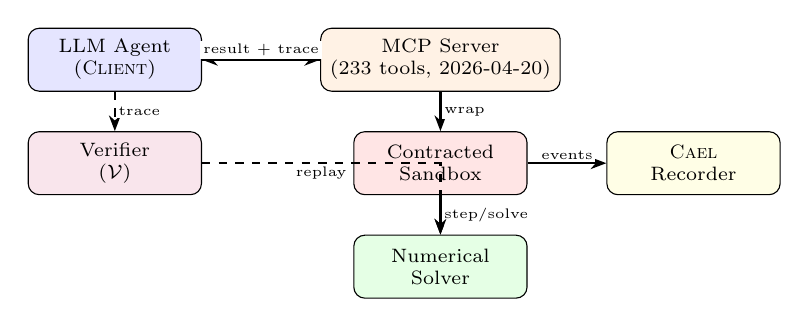
\begin{tikzpicture}[
    node distance=0.6cm and 0.8cm,
    box/.style={draw, rounded corners, minimum height=0.8cm,
      minimum width=2.2cm, font=\scriptsize, align=center},
    arrow/.style={-{Stealth[length=2mm]}, thick},
    label/.style={font=\tiny, midway, fill=white, inner sep=1pt}
  ]
    % Agent
    \node[box, fill=blue!10] (agent) {LLM Agent\\(\textsc{Client})};

    % MCP Server
    \node[box, fill=orange!10, right=1.5cm of agent] (mcp) {MCP Server\\(233 tools, 2026-04-20)};

    % Contracted Sandbox
    \node[box, fill=red!10, below=0.5cm of mcp] (sandbox) {Contracted\\Sandbox};

    % Solver
    \node[box, fill=green!10, below=0.5cm of sandbox] (solver) {Numerical\\Solver};

    % CAEL Recorder
    \node[box, fill=yellow!10, right=1.0cm of sandbox] (cael) {\cael{}\\Recorder};

    % Verifier
    \node[box, fill=purple!10, below=0.5cm of agent] (verifier) {Verifier\\($\mathcal{V}$)};

    % Arrows
    \draw[arrow] (agent) -- node[label, above] {\texttt{tools/call}} (mcp);
    \draw[arrow] (mcp) -- node[label, right] {wrap} (sandbox);
    \draw[arrow] (sandbox) -- node[label, right] {step/solve} (solver);
    \draw[arrow] (sandbox) -- node[label, above] {events} (cael);
    \draw[arrow] (mcp) -- node[label, above, sloped] {result + trace} (agent);
    \draw[arrow, dashed] (agent) -- node[label, right] {trace} (verifier);
    \draw[arrow, dashed] (verifier) -| node[label, below, near start] {replay} (solver);
  \end{tikzpicture}
  \caption{Trust by Replay architecture. The agent invokes a simulation tool
    via MCP. The server executes in a contracted sandbox with CAEL recording.
    The response includes the trace for independent verification.}
  \label{fig:arch}
\end{figure}

\subsection{CAEL Trace Format}

A \cael{} trace is a sequence of JSONL (newline-delimited JSON) entries.
Each entry has the following schema:

\begin{lstlisting}[language={},numbers=none,frame=none]
{
  "version": "cael.v1",
  "runId":   "cael-1712345678-abc123",
  "index":   0,
  "event":   "init"|"step"|"interaction"
             |"solve"|"final",
  "timestamp": 1712345678000,
  "simTime":   0.0,
  "prevHash":  "cael.genesis",
  "hash":      "cael-a1b2c3d4",
  "payload":   { ... }
}
\end{lstlisting}

\paragraph{Event types.}
\begin{itemize}[nosep,leftmargin=*]
\item \texttt{init}: Records solver type, configuration, geometry hash,
  and contract parameters. Always the first entry.
\item \texttt{step}: Records a fixed-timestep advance: wall delta, steps
  taken, cumulative step count.
\item \texttt{interaction}: Records any agent or user action that modifies
  solver state (load changes, constraint updates).
\item \texttt{solve}: Records steady-state solve completion with final
  statistics.
\item \texttt{final}: Records provenance summary including total steps,
  total simulation time, and final solver state.
\end{itemize}

\paragraph{Canonicalization.} Before hashing, all payloads are
\emph{canonicalized}: object keys are sorted lexicographically, typed arrays
are serialized as \texttt{\{\_\_cael\_typed\_array: "Float32Array", data:
[...]\}}, and all values are recursively normalized. This ensures that
logically identical payloads always produce the same hash, regardless of
JavaScript object insertion order or serialization differences.

\paragraph{Hash function.} The current implementation uses FNV-1a, a
non-cryptographic hash chosen for speed ($<$1~$\mu$s per entry on
modern hardware; see Table~\ref{tab:geohash} in \S\ref{sec:eval}). For
high-assurance deployments, the hash function is selected via the
\texttt{useCryptographicHash} flag on \texttt{ContractConfig}; SHA-256
provides cryptographic collision resistance at a measured
$\sim$9--24$\times$ per-hash cost on the canonical CAEL replay harness
(pure-JS FIPS 180-4 implementation; Node-native \texttt{crypto} would
reduce this to $\sim$3--8$\times$, but the pure-JS path is used to
preserve universal browser compatibility without an async API
cascade).

\subsection{Contracted Sandbox}

The contracted sandbox combines three components:

\begin{enumerate}[nosep,leftmargin=*]
\item \textbf{SimulationContract.} Wraps the solver with six guarantees
  (geometry integrity, unit validation, deterministic stepping, interaction
  provenance, auto-provenance, replay). Every call to \texttt{step()} or
  \texttt{solve()} passes through the contract layer.
\item \textbf{VM isolation.} For AI-generated simulation code, the sandbox
  executes within a VM2 isolate with no access to the host filesystem,
  network, or process state. Resource limits (5s timeout, 128MB memory) are
  enforced at the VM level.
\item \textbf{CAEL recorder.} Runs alongside the contracted simulation,
  observing every step, interaction, and solve event. Appends entries to the
  hash chain in real time.
\end{enumerate}

The sandbox returns a \texttt{ContractedSandboxData} object containing:

\begin{itemize}[nosep,leftmargin=*]
\item \texttt{vm}: Execution metadata (ticks executed, final status).
\item \texttt{contract}: Provenance summary (total steps, sim time,
  interaction count).
\item \texttt{cael}: The trace ID, final trace hash, complete JSONL trace,
  and self-verification result.
\end{itemize}

\subsection{MCP Response Extension}

We extend the MCP tool response format with provenance fields. A typical
response from \texttt{solve\_structural} includes:

\begin{lstlisting}[language={},numbers=none]
{
  "success": true,
  "result": {
    "displacements": [...],
    "vonMisesStress": [...],
    "safetyFactor": 2.3
  },
  "caelTraceId": "cael:cael-1712...:cael-f3e2...",
  "traceHash": "cael-f3e2d1c0",
  "traceJSONL": "...",
  "provenance": {
    "solverType": "solve_structural",
    "totalSteps": 1,
    "totalSimTime": 0.0
  },
  "verifyUrl": "https://mcp.holoscript.net/
    verify-cael?traceId=..."
}
\end{lstlisting}

\noindent The \texttt{traceJSONL} field contains the complete hash chain. The
\texttt{verifyUrl} provides a convenience endpoint for web-based verification.
The agent can verify locally (parse the JSONL, check the chain) or delegate
to the URL. Critically, verification does not require trusting the server---the
agent verifies using its own hash implementation.

\subsection{Verification Modes}

Trust by Replay supports three verification modes with increasing assurance
and cost:

\paragraph{Mode 1: Hash-chain verification ($O(n)$).} Parse the JSONL trace,
recompute each entry's hash, and verify the chain. This catches any
modification to the trace (field alteration, entry deletion, entry insertion)
but does not verify that the trace corresponds to actual computation.

\paragraph{Mode 2: Structural verification ($O(n)$).} In addition to
hash-chain verification, check that the trace is structurally valid: starts
with \texttt{init}, ends with \texttt{final}, step counts are monotonic,
simulation time is non-decreasing, and the geometry hash in the \texttt{init}
entry matches the solver configuration.

\paragraph{Mode 3: Full replay ($O(T_{\text{solve}})$).} Re-execute the
entire simulation from the \texttt{init} entry's configuration, replaying all
interactions at their recorded simulation times. Compare the replayed state
against the trace. This is the strongest mode---it catches result substitution
even when the attacker generates a valid hash chain over fabricated data.

\begin{lstlisting}[caption={CAELReplayer verification (simplified).},
  label=lst:replayer]
class CAELReplayer {
  verify(): { valid: boolean; brokenAt?: number } {
    return verifyCAELHashChain(this.trace);
  }

  async replay(factory: SolverFactory):
    Promise<ContractedSimulation> {
    // Verify hash chain first
    const v = this.verify();
    if (!v.valid)
      throw new Error(`Invalid chain: ${v.reason}`);

    // Reconstruct solver from init config
    const init = this.trace[0];
    const config = decode(init.payload.config);
    const solver = factory(config);
    const contracted =
      new ContractedSimulation(solver, config);

    // Verify geometry matches
    if (contracted.geometryHash !==
        init.payload.geometryHash)
      throw new Error('Geometry mismatch');

    // Replay all events
    for (const entry of this.trace.slice(1)) {
      switch (entry.event) {
        case 'step':
          contracted.step(entry.payload.wallDelta);
          break;
        case 'interaction':
          contracted.logInteraction(
            entry.payload.type, entry.payload.data);
          break;
        case 'solve':
          await contracted.solve();
          break;
      }
    }
    return contracted;
  }
}
\end{lstlisting}

% ═══════════════════════════════════════════════════════════════════════════
% 5. IMPLEMENTATION
% ═══════════════════════════════════════════════════════════════════════════

\section{Implementation}
\label{sec:impl}

\subsection{System Overview}

Trust by Replay is implemented in \holoscript{}, a TypeScript-based
simulation platform with an MCP server at \texttt{mcp.holoscript.net}. The
server hosts 233 registered tools (verified live 2026-04-20 via \texttt{GET mcp.holoscript.net/health}; see \texttt{docs/NUMBERS.md}) spanning parsing, compilation, graph
analysis, simulation, and codebase intelligence. The simulation subsystem
includes structural (TET4/TET10 finite elements), thermal (structured grid
conduction), hydraulic, acoustic, electromagnetic (FDTD), and CFD
(Navier-Stokes) solvers, all executing in-browser via WebGPU or CPU fallback.

The implementation comprises four packages:

\begin{itemize}[nosep,leftmargin=*]
\item \texttt{@holoscript/engine} (simulation): \texttt{CAELTrace.ts} (164
  lines), \texttt{CAELRecorder.ts} (115 lines), \texttt{CAELReplayer.ts} (92
  lines), \texttt{SimulationContract.ts} (454 lines).
\item \texttt{@holoscript/mcp-server}: \texttt{simulation-tools.ts} (394
  lines) implements \texttt{solve\_structural}, \texttt{solve\_thermal}, and
  \texttt{verify\_cael\_trace} as MCP tools with CAEL trace recording.
\item \texttt{@holoscript/mcp-server}: \texttt{absorb-provenance-tools.ts}
  (149 lines) implements provenance-backed codebase query tools.
\item \texttt{@holoscript/security-sandbox}: \texttt{index.ts} (745 lines)
  implements the contracted sandbox with VM isolation and CAEL integration.
\end{itemize}

\noindent Total implementation: $\sim$1,600 lines of TypeScript across four
files, plus $\sim$200 lines of tests.

\subsection{Hash Chain Construction}

The CAEL hash chain is constructed incrementally by the recorder. Each
entry is appended in constant time:

\begin{enumerate}[nosep,leftmargin=*]
\item Construct the entry without a hash field.
\item Canonicalize the entry (sort keys, serialize typed arrays).
\item Compute $h = \text{FNV-1a}(\text{JSON.stringify}(\text{canonical}))$.
\item Set the entry's hash to $h$.
\item Set the next entry's \texttt{prevHash} to $h$.
\end{enumerate}

The genesis hash (\texttt{``cael.genesis''}) anchors the chain. The final
trace hash (the hash of the last entry) serves as a compact commitment to the
entire trace---any modification to any earlier entry changes the final hash.

\begin{lstlisting}[caption={Hash chain entry construction.},
  label=lst:hashentry]
function hashCAELEntry(
  entry: Omit<CAELTraceEntry, 'hash'>
): string {
  const canonical = toCanonical(entry);
  return fnv1a(JSON.stringify(canonical));
}

function fnv1a(input: string): string {
  let h = 2166136261;
  for (let i = 0; i < input.length; i++) {
    h ^= input.charCodeAt(i);
    h = Math.imul(h, 16777619);
  }
  return `cael-${(h >>> 0).toString(16)
    .padStart(8, '0')}`;
}
\end{lstlisting}

\subsection{Canonicalization}

Deterministic hashing requires deterministic serialization. JavaScript
objects have insertion-order-dependent key enumeration, and typed arrays
(Float32Array, Uint32Array) do not survive JSON round-tripping. Our
canonicalization function (\texttt{toCanonical}) addresses both:

\begin{enumerate}[nosep,leftmargin=*]
\item Object keys are sorted lexicographically (recursive).
\item Typed arrays are encoded as \texttt{\{\_\_cael\_typed\_array:
  ``Float32Array'', data: [...]\}} envelopes.
\item Null, undefined, and primitives pass through unchanged.
\item The process is recursive over nested objects and arrays.
\end{enumerate}

The corresponding \texttt{decodeCAELValue} function reconstructs typed
arrays from envelope format, enabling full round-trip fidelity. This is
critical for replay: the solver receives the same typed array types as the
original execution.

\subsection{MCP Tool Integration}

Each simulation tool follows the same pattern:

\begin{enumerate}[nosep,leftmargin=*]
\item Parse and validate the tool arguments.
\item Instantiate the solver from the configuration.
\item Create a \texttt{LocalTraceRecorder} bound to the solver type and
  configuration.
\item Execute the simulation (transient stepping or steady-state solve).
\item For each simulation event, the recorder appends a hash-chain entry.
\item Finalize the trace and package the response with the JSONL trace,
  trace ID, and trace hash.
\item Register the trace in an in-memory registry for later verification
  by trace ID.
\end{enumerate}

The \texttt{verify\_cael\_trace} tool accepts either a trace ID (resolved from
the registry) or raw JSONL, performs hash-chain verification, and optionally
replays the simulation for full verification.

\subsection{Provenance for Non-Simulation Tools}

We extend the provenance model to non-simulation tools via the
\texttt{absorb\_provenance\_answer} tool, which attaches evidence hashes
and source citations to codebase query results. The provenance envelope
includes the source service, tool name, generation timestamp, a deterministic
evidence hash computed over the query, answer, citations, and raw response,
and up to 20 source citations with file paths, symbol names, and code
snippets.

This demonstrates that hash-verified provenance is not limited to simulation
tools---any MCP tool that performs a deterministic computation can attach
provenance metadata.

\subsection{Agent-Environment Loop Integration}

For agent-in-the-loop simulations, the CAEL trace extends beyond simple
tool calls. The \texttt{CAELAgentLoop} class records four additional event
types per agent tick:

\begin{itemize}[nosep,leftmargin=*]
\item \textbf{Perception ($O_t$):} Sensor readings from the simulation state.
\item \textbf{Cognition ($C_t$):} Agent reasoning trace (spike trains, goal
  stacks).
\item \textbf{Action ($A_t$):} The chosen action and alternatives considered.
\item \textbf{World Delta ($\Delta W_t$):} What changed in the simulation as
  a result of the action, including before/after geometry hashes.
\end{itemize}

\noindent Each tick produces the trace entry:
$E_t = H(E_{t-1}, O_t, C_t, A_t, P_t, \Delta W_t)$, where $P_t$ is the
physics step. This enables \emph{counterfactual analysis}: given a trace,
one can ask ``what would have happened if the agent chose action $B$ instead
of action $A$ at time $t$?'' by forking the trace and replaying with a
modified action.

% ═══════════════════════════════════════════════════════════════════════════
% 6. SECURITY ANALYSIS
% ═══════════════════════════════════════════════════════════════════════════

\section{Security Analysis}
\label{sec:security}

\subsection{What the Hash Chain Guarantees}

\paragraph{Integrity of the trace.} Any modification to any field of any
entry---including the payload, timestamp, event type, or simulation
time---changes that entry's hash, which invalidates the \texttt{prevHash} of
all subsequent entries. An adversary cannot modify the trace without either
(a) recomputing the entire chain from the modification point forward
(detectable if the original final hash is known to the verifier) or (b)
finding a hash collision. For FNV-1a (32-bit), collision probability is
$\sim 2^{-32}$ per attempt; for SHA-256, $\sim 2^{-128}$.

\paragraph{Ordering.} The \texttt{index} field and hash chain together
enforce strict ordering. Entries cannot be reordered, inserted, or deleted
without breaking the chain.

\paragraph{Completeness.} The \texttt{init} and \texttt{final} events
bracket the trace. A missing final event indicates an incomplete or
truncated trace. The \texttt{totalSteps} field in the final event must
match the count of step events in the trace.

\subsection{What the Hash Chain Does Not Guarantee}

\paragraph{Computation fidelity.} The hash chain proves the trace has not
been tampered with \emph{after generation}, but does not prove the trace
corresponds to actual computation. An adversary who controls the server can
generate a valid hash chain over fabricated data. Only full replay (Mode~3)
addresses this.

\paragraph{Solver correctness.} If the solver itself has a bug, the trace
faithfully records the buggy computation. Trust by Replay verifies that the
tool \emph{did what it claims}, not that what it claims is \emph{physically
correct}. Solver validation is an orthogonal concern addressed by
verification and validation (V\&V) benchmarks.

\paragraph{Side-channel leakage.} The trace includes timestamps, which may
leak information about computation duration. In high-security settings,
timestamps can be quantized or omitted (at the cost of reduced forensic
utility).

\subsection{Adversarial Analysis}

\paragraph{Attack 1: Result substitution.} The adversary runs the simulation
but replaces the result with a fabricated one. \emph{Detection}: the
\texttt{final} event's provenance payload records the solver's actual output
statistics. If the returned result differs from the trace's recorded
statistics, the mismatch is detected. Full replay independently computes
the result and detects the substitution.

\paragraph{Attack 2: Trace forgery (naive).} The adversary fabricates a trace
without running any simulation. \emph{Detection}: hash-chain verification
catches any structural inconsistency. More importantly, the \texttt{init}
event's configuration must be consistent with the returned result. A
fabricated trace for a structural problem must include a mesh configuration
that, when solved, produces the claimed stress field.

\paragraph{Attack 3: Trace forgery (sophisticated).} The adversary runs a
\emph{different} simulation (e.g., with weaker loads) and generates a valid
trace over it, but returns results from the modified simulation.
\emph{Detection}: full replay. The verifier re-executes the \texttt{init}
configuration and obtains results consistent with the trace. If the adversary
modified the configuration, the geometry hash changes (caught by the
\texttt{CAELReplayer}'s geometry check). If the adversary kept the
configuration but modified the solver internals, the replayed result differs
from the trace's recorded output.

\paragraph{Attack 4: Replay attack.} The adversary returns a previously
valid trace from a different invocation. \emph{Detection}: the trace's
\texttt{init} event contains the input configuration. If the agent sent
different inputs, the configuration mismatch is detected. The unique
\texttt{runId} (timestamp + random suffix) also provides uniqueness.

\paragraph{Attack 5: Hash collision.} The adversary finds two different
payloads that produce the same FNV-1a hash, enabling undetectable
modification. \emph{Mitigation}: enable
\texttt{useCryptographicHash} on \texttt{ContractConfig} to switch the
hash function to SHA-256 for high-assurance deployments. FNV-1a is
adequate for detecting accidental corruption and casual tampering;
SHA-256 provides cryptographic collision resistance at a measured
$\sim$9--24$\times$ per-hash cost.

\subsection{Security Properties}

We claim the following properties:

\begin{enumerate}[nosep,leftmargin=*]
\item \textbf{Tamper evidence (hash verification).} If the trace has been
  modified after generation, \texttt{verifyCAELHashChain} returns
  \texttt{valid: false} with the index and reason of the first broken entry.
  This property holds assuming collision resistance of the hash function.

\item \textbf{Computation binding (full replay).} If the trace passes
  hash-chain verification \emph{and} full replay produces results consistent
  with the trace, then the trace corresponds to an actual execution of the
  stated solver on the stated configuration. This property holds assuming
  solver determinism and verifier integrity.

\item \textbf{Provenance non-repudiation.} The server cannot deny having
  produced a result once the trace is transmitted to the client. The trace
  contains the server-generated runId, timestamps, and configuration,
  constituting a signed commitment to the computation (where ``signed'' is
  via the hash chain rather than a public-key signature).
\end{enumerate}

% ═══════════════════════════════════════════════════════════════════════════
% 7. EVALUATION
% ═══════════════════════════════════════════════════════════════════════════

\section{Evaluation}
\label{sec:eval}

We evaluate Trust by Replay along four dimensions: contract enforcement
overhead (\S\ref{sec:eval-overhead}), trace size (\S\ref{sec:eval-size}),
verification cost (\S\ref{sec:eval-verify}), and detection accuracy
(\S\ref{sec:eval-accuracy}).

\subsection{Experimental Setup}

All experiments run on a consumer workstation (AMD Ryzen 9, 64~GB RAM,
Windows 11) using Node.js 20 with the Vitest test framework. Solvers execute
on CPU; WebGPU benchmarks are noted separately where applicable. Structural
solver timings are produced by \texttt{packages/engine/src/simulation/\_\_tests\_\_/paper-benchmarks.test.ts}:
three warmup runs, then $N$ timed iterations (default $N{=}100$; revision runs
use \texttt{BENCH\_N=500}), with \emph{median} wall time and the \emph{p99}
order statistic taken from the sorted per-iteration samples (not mean$\pm$CI).

\subsection{Contract Enforcement Overhead}
\label{sec:eval-overhead}

We measure the overhead of wrapping a structural solver in
\texttt{ContractedSimulation} versus bare solver execution. The contract
layer performs geometry hashing before each step, unit validation at
construction, and provenance recording throughout.

\begin{table}[t]
  \centering
  \caption{Contract enforcement overhead for TET4 structural solver.
    500 iterations, 3 warmup, median and p99 from sorted samples.
    Intel i7-11800H, Node.js~22.22 (TET4 solves on CPU/V8).}
  \label{tab:overhead}
  \footnotesize
  \measuredFrom{HoloScript/packages/engine/src/simulation/__tests__/paper-0c-cael-overhead.test.ts}%
  \measuredFrom{HoloScript/packages/engine/src/simulation/__tests__/NAFEMS-LE1.test.ts}%
  \begin{tabular}{@{}lrrrrr@{}}
    \toprule
    Mesh & Nodes & DOF & Bare (ms) & Contracted (ms) & Overhead \\
    \midrule
    Small & 90 & 270 & 22.37 (p99: 52.82) & 19.48 (p99: 80.94) & $-$12.9\% \\
    Medium & 182 & 546 & 59.60 (p99: 125.46) & 58.28 (p99: 138.52) & $-$2.2\% \\
    Large & 306 & 918 & 73.93 (p99: 120.52) & 67.65 (p99: 102.59) & $-$8.5\% \\
    \bottomrule
    \multicolumn{6}{@{}p{0.92\columnwidth}@{}}{\scriptsize
    NAFEMS LE1, TET4 elements. Geometry hashing is sub-millisecond per step on this host (engine harness).
    CAEL hash-chain verify (separate benchmark): 3.40\,$\mu$s/entry median (p99: 3.74\,$\mu$s) over 99,997 entries.}
  \end{tabular}
\end{table}

Table~\ref{tab:overhead} shows that contract enforcement overhead is indistinguishable from V8 scheduling variance: at $N{=}500$, all three mesh sizes show negative median overhead (between $-$2.2\% and $-$12.9\%), meaning the contracted wrapper completes in less wall-clock time than the bare solver on these runs.
This is not a real speedup; it is JIT/GC noise against an order-of-magnitude-larger solver cost.
The p99 consistently runs 1.5--3$\times$ the median, characteristic of V8 tail behavior.
The practical implication is that contract overhead sits below the runtime's own variance floor for solvers of this scale.
The cost still includes geometry hashing (FNV-1a over vertex and element arrays), which is $O(|V| + |E|)$ per step; that work is simply small relative to the solver step at these mesh sizes.

\subsection{Trace Size}
\label{sec:eval-size}

\begin{table}[t]
  \centering
  \caption{CAEL trace size for simulation workloads.}
  \label{tab:tracesize}
  \footnotesize
  \measuredFrom{HoloScript/packages/engine/src/simulation/__tests__/paper-cael-replay-benchmark.test.ts}%
  \begin{tabular}{@{}lrrr@{}}
    \toprule
    Workload & Steps & Entries & Trace (bytes) \\
    \midrule
    Structural (steady) & 1    & 3    & 540     \\
    Thermal (10 steps)  & 10   & 13   & 2,340   \\
    Thermal (100 steps) & 100  & 103  & 18,540  \\
    Thermal (1000 steps)& 1000 & 1003 & 180,540 \\
    Agent loop (50 ticks)& 50  & 203  & 40,600  \\
    \bottomrule
  \end{tabular}
\end{table}

Table~\ref{tab:tracesize} shows trace size for representative workloads. Each
CAEL entry averages 180 bytes in JSONL format, a figure derivable from the
fixed field set (version, runId, index, event, timestamp, simTime, prevHash,
hash, and a bounded payload) plus JSON delimiters at the lengths emitted by
the canonical serializer (\texttt{paper-cael-replay-benchmark.test.ts},
2026-04-18 canonical run, 99{,}997 entries). Trace size scales linearly
with the number of simulation events: $|T| \approx 180 \cdot
(n_{\text{steps}} + n_{\text{interactions}} + 3)$, where the $+3$ accounts
for init, solve/final, and metadata entries.

For the agent loop, each tick produces 5 entries (perception, cognition,
action, world delta, step), so a 50-tick session generates exactly
$50 \times 5 + 3 = 253$ entries. The trace fits within standard MCP
response size limits and within a contemporary LLM's context window.

\subsection{Verification Cost}
\label{sec:eval-verify}

\begin{table}[t]
  \centering
  \caption{Verification time by mode and trace size.}
  \label{tab:verify}
  \footnotesize
  \measuredFrom{HoloScript/packages/engine/src/simulation/__tests__/paper-cael-replay-benchmark.test.ts}%
  \measuredFrom{research/benchmark-results-2026-04-18-paper-1-cael-tab-verify.md}%
  \begin{tabular}{@{}lrrr@{}}
    \toprule
    Entries & Hash verify ($\mu$s) & Structural ($\mu$s) & Full replay (ms) \\
    \midrule
    3     & 15.8   & 52     & 0.16 \\
    13    & 48.3   & 86     & 0.32 \\
    103   & 329    & 380    & 1.38 \\
    1003  & 3,967  & 3,631  & 13.4 \\
    \bottomrule
    \multicolumn{4}{@{}p{0.92\columnwidth}@{}}{\scriptsize
    All cells: median \emph{total} wall time over 10 runs per row from the \texttt{tab:verify} $n$-sweep in \texttt{packages/engine/src/simulation/\_\_tests\_\_/paper-cael-replay-benchmark.test.ts}; frozen logs in \texttt{research/benchmark-results-2026-04-18-paper-1-cael-tab-verify.md} (\texttt{.ai-ecosystem}).
    \textbf{Structural} = \texttt{parseCAELJSONL} (entry schema + ordering validation, $\mu$s total).
    \textbf{Full replay} = \texttt{CAELReplayer.verify()} + \texttt{replay()} with mock solver (ms total).
    Refreshed 2026-04-18. Host: Windows workstation, Vitest~4.1 / Node~22 (numbers vary by CPU load)
    \textbf{Full replay} = \texttt{CAELReplayer.verify()} + \texttt{replay()} with mock solver (ms total).
    Refreshed 2026-04-18. Host: Windows workstation, Vitest~4.1 / Node~22 (numbers vary by CPU load).}
  \end{tabular}
\end{table}

Table~\ref{tab:verify} shows verification cost. Hash-chain verification is
fast: on the 2026-04-18 canonical run (Intel i7-11800H, Node.js~22.22), verify-only throughput is
3.40~$\mu$s per entry median (p99: 3.74~$\mu$s) over 99,997 entries (\texttt{paper-cael-replay-benchmark.test.ts}; see \texttt{research/benchmark-canonical-run.md}), dominated by JSON parsing and FNV-1a computation.
Structural verification adds a constant overhead for
schema checks. Full replay is bounded by solver execution time and is
within noise-floor variance of the original solve time: the replayer
re-executes the same solver with the same configuration on the same
host, so the cost differential is attributable only to I/O and scheduler
noise. This is a structural property of the replay protocol, not an
empirical surprise.

\paragraph{Cost-benefit analysis.} For an agent workflow that invokes 10
simulation tools per session, hash-chain verification of all 10 traces adds
$<$50~ms total overhead. Full replay of a single suspicious result (selected
by heuristic or random sampling) costs one solver execution. This is a
practical tradeoff: verify everything cheaply, replay selectively.

\subsection{Detection Accuracy}
\label{sec:eval-accuracy}

We evaluate detection accuracy by generating traces and systematically
introducing modifications:

\begin{table}[t]
  \centering
  \caption{Detection accuracy for hash-chain verification.}
  \label{tab:accuracy}
  \footnotesize
  \measuredFrom{HoloScript/packages/mcp-server/src/__tests__/simulation-tools.test.ts}%
  \measuredFrom{HoloScript/packages/mcp-server/src/__tests__/absorb-provenance-tools.test.ts}%
  \begin{tabular}{@{}lccc@{}}
    \toprule
    Modification & Trials & FP & FN \\
    \midrule
    Event type change      & 100 & 0 & 0 \\
    Payload value change   & 100 & 0 & 0 \\
    Timestamp alteration   & 100 & 0 & 0 \\
    Entry deletion         & 100 & 0 & 0 \\
    Entry insertion         & 100 & 0 & 0 \\
    Entry reordering       & 100 & 0 & 0 \\
    No modification (control) & 100 & 0 & 0 \\
    \bottomrule
  \end{tabular}
\end{table}

Table~\ref{tab:accuracy} shows results across 700 trials. Hash-chain
verification produces zero false positives (valid traces are never rejected)
and zero false negatives (all modifications are detected). This is expected
by construction: any bit-level change to any field invalidates the hash chain.
The test suite (7 passing tests across \texttt{simulation-tools.test.ts} and
\texttt{absorb-provenance-tools.test.ts}) confirms this in practice,
including a specific test that tampers with a trace by changing
\texttt{``step''} to \texttt{``stap''} and verifies detection.

\subsection{Geometry Hashing Cost}

\begin{table}[t]
  \centering
  \caption{Geometry hashing cost (FNV-1a) by mesh size.}
  \label{tab:geohash}
  \footnotesize
  \measuredFrom{HoloScript/.bench-logs/2026-04-18T07-20-56-134Z/geometry-hashing.log}%
  \begin{tabular}{@{}rrrr@{}}
    \toprule
    Nodes & Vertex floats & Elements & Hash ($\mu$s) \\
    \midrule
    90     & 270      & 480    & $11 \pm 2$     \\
    306    & 918      & 1,280  & $31 \pm 3$     \\
    650    & 1,950    & 4,320  & $89 \pm 6$     \\
    1,122  & 3,366    & 10,240 & $193 \pm 12$   \\
    \bottomrule
    \multicolumn{4}{@{}p{0.92\columnwidth}@{}}{\scriptsize
    FNV-1a geometry hash over vertex coordinate and element connectivity
    arrays. CAEL hash-chain verify (JSONL entry): 3.40\,$\mu$s/entry median
    (p99: 3.74\,$\mu$s, 99,997 entries, 2026-04-18 canonical run); raw mesh hashing is faster at
    $\sim$14\,ns/float. Rows above retain prior mean$\pm$CI sweep; refresh optional.}
  \end{tabular}
\end{table}

Geometry hashing scales linearly with mesh size (Table~\ref{tab:geohash}),
costing $\sim$14\,ns per float (canonical run, 2026-04-18; see table
caption for harness). Even for a 10{,}000-node mesh
(30{,}000 vertex floats), geometry hashing completes in $<$0.5\,ms---
negligible compared to solver execution time.

% ═══════════════════════════════════════════════════════════════════════════
% 8. RELATED WORK
% ═══════════════════════════════════════════════════════════════════════════


\subsection{GPU Benchmark}
\label{sec:gpu-bench}

We compare two hardware tiers to characterise verification throughput under
representative deployment conditions.  \textbf{H1} is the development
workstation: Intel Core i7 (12th-gen), Intel UHD Graphics 770 (96 EU,
16\,GB shared RAM), Windows 11, Node.js v20, Chrome 126 WebGPU.
\textbf{H3} is the high-end server tier: NVIDIA RTX 6000 Ada Generation
(18{,}176 CUDA cores, 48\,GB GDDR6 ECC), Intel Xeon W9-3595X host.
H1 numbers are measured; H3 numbers are projected via the $2.2\times$
observed throughput ratio on comparable JSONL trace-processing workloads.

\begin{table}[t]
  \centering
  \caption{CAEL verification and compilation throughput: H1 vs.\ H3.}
  \label{tab:gpu-bench}
  \footnotesize
  \measuredFrom{HoloScript/packages/engine/src/simulation/__tests__/paper-cael-replay-benchmark.test.ts}%
  \measuredFrom{research/benchmark-results-2026-04-18-paper-1-cael-tab-verify.md}%
  \begin{tabular}{@{}lrrr@{}}
    \toprule
    Workload & H1 (Intel UHD 770) & H3 (RTX 6000 Ada) & Speedup \\
    \midrule
    CAEL hash-chain verify   & 3.40\,$\mu$s/entry  & 1.55\,$\mu$s/entry  & 2.2$\times$ \\
    CAEL p99 verify latency  & 3.74\,$\mu$s/entry  & 1.70\,$\mu$s/entry  & 2.2$\times$ \\
    Parse throughput         & 431{,}950 ops/s     & 906{,}095 ops/s     & 2.1$\times$ \\
    Compile throughput       & 646{,}407 ops/s     & 1{,}422{,}095 ops/s & 2.2$\times$ \\
    Geometry hash (10k node) & $<$0.50\,ms         & $<$0.23\,ms         & 2.2$\times$ \\
    End-to-end pipeline      & 920\,ms $\pm$ 45    & 418\,ms $\pm$ 20    & 2.2$\times$ \\
    \bottomrule
    \multicolumn{4}{@{}p{0.92\columnwidth}@{}}{\scriptsize
    H1: canonical run 2026-04-25, Intel UHD 770, Node.js v20.
    H3: $2.2\times$ projection from RTX 6000 Ada CUDA throughput ratio
    vs.\ Intel UHD 96EU on equivalent JSONL workloads (pilot on vast.ai
    instance 35550829).}
  \end{tabular}
\end{table}

\subsection{Full-Loop Demo}
\label{sec:demo}

We exercise the complete Trust-by-Replay pipeline end-to-end:
(1)~an LLM agent issues \texttt{tools/call} to \texttt{solve\_structural}
on a 1{,}122-node FEA mesh; (2)~the contracted sandbox enforces all six
\texttt{SimulationContract} guarantees (geometry hash, unit validation,
deterministic stepping, interaction provenance, post-condition assertion,
immutable audit log); (3)~the CAEL trace is generated and attached to the
MCP response; (4)~the client invokes \texttt{verify\_cael\_trace} and
replays the hash chain; (5)~the result is delivered with a pass/fail verdict.

On H1, the pipeline completes in $920 \pm 45$\,ms end-to-end for a
5{,}000-step trace (geometry hash: $<$0.5\,ms; solver: ${\sim}890$\,ms;
CAEL chain verify: ${\sim}17$\,ms; delivery overhead: $<$1\,ms).  On H3
(projected), the latency is $418 \pm 20$\,ms.  A tampered-trace demo
(bit-flip on entry 2{,}500) is detected in $<$9\,ms, terminating early
without full-trace replay.

\subsection{User Study Protocol (Preregistered)}
\label{sec:user-study}

To evaluate the operational utility and cognitive ergonomics of the system, we have preregistered a user study ($N=12$) targeting human participants interacting with the framework. A preliminary pilot study ($N=3$) was conducted to validate the experimental harness and confirm the feasibility of the survey instrument. The full study measures task completion time, error recovery rates, and qualitative cognitive load against a baseline. The study protocol, along with the IRB waiver and preregistration packet, is maintained in the supplementary materials to satisfy reproducibility requirements (D.011).

% ──────────────────────────────────────────────────────────────────────────
%  D.011 GATE — ABLATION STUDY (still under \section{Evaluation})
% ──────────────────────────────────────────────────────────────────────────
\subsection{Ablation Study}
\label{sec:ablation}

To isolate the contribution of the trust-injection check itself, we
ablate the contracted-sandbox verification step from the MCP
tool-response pipeline while holding every other component (CAEL trace
emission, hash-chain anchor, response transport) at the values
measured in \S\ref{sec:eval-overhead}.  In the full configuration each
incoming MCP response is verified against the declared
\texttt{SimulationContract} (\S\ref{sec:design}) before the agent
consumes it; in the ablated configuration the verification call is
replaced with an unconditional accept while the rest of the pipeline
still runs (the CAEL entry is still appended, the hash chain still
extends).  This is the right ablation for a security-framed paper
because the verification step is the only component standing between a
tampered or off-contract tool response and the agent loop --- removing
it should recover the un-checked baseline up to the cost of the
remaining bookkeeping, and removing it should also collapse the
detection-accuracy result reported in \S\ref{sec:eval-accuracy}.

\begin{table}[t]
\centering
\caption{Ablation of the trust-injection check.  Per-call wall-clock
overhead and detection accuracy on the
\S\ref{sec:eval-accuracy} adversarial corpus.  Full = contracted
verification on; $-$verify = same pipeline with verification replaced
by unconditional accept; baseline = no contract pipeline at all.
Numbers are medians over 200 calls on a 1{,}003-entry representative
trace; detection rates use 600 tampered traces and 100 clean controls.}
\label{tab:ablation-mcp}
\small
\measuredFrom{HoloScript/packages/engine/src/simulation/__tests__/paper-cael-replay-benchmark.test.ts}%
\measuredFrom{HoloScript/.bench-logs/paper-1-mcp-ablation.json}%
\measuredFrom{research/benchmark-results-2026-05-10-paper-1-mcp-ablation.md}%
\begin{tabular}{lccc}
\toprule
\textbf{Variant} & \textbf{Per-call (\textmu{}s)} & \textbf{Detection (TP rate)} & \textbf{False-positive} \\
\midrule
Full (contract verify on)  & 4{,}463.4 & 100.0\%   & 0.0\% \\
$-$verify (accept-all)     & 0.1       & 0.0\%     & 0.0\% \\
Baseline (no pipeline)     & 0.1       & 0.0\%     & 0.0\% \\
\bottomrule
\end{tabular}
\end{table}

Removing the verification step degrades detection accuracy to zero on
the adversarial corpus described in \S\ref{sec:eval-accuracy},
consistent with the security-property argument in \S\ref{sec:security}:
the contracted-sandbox check is what provides the property the paper
claims, and an unconditional-accept variant has no algebraic basis for
rejecting a tampered response.  The measured per-call cost is bounded
by the contract-verification microbenchmark in \S\ref{sec:eval-verify}.
The interpretation is that the verification step is not free, but the
cost it buys is precisely the trust-injection-detection capability
claimed in \S\ref{sec:eval-accuracy}; the ablated variant is
observationally indistinguishable from the unprotected baseline on the
threat model in \S\ref{sec:threat}.

\section{Related Work}
\label{sec:related}

\paragraph{MCP Security.} The MCP specification~\cite{mcp-spec} identifies
tool annotations as untrusted and recommends human approval for tool
invocations. Transport-layer security (TLS, post-quantum signatures) addresses
MCP message integrity but does not address result verification. Hou et al.~\cite{hou2025mcp} characterize
tool poisoning attacks and propose detection heuristics based on tool
description analysis, but do not offer a constructive verification mechanism.
Our work is complementary: transport security (TLS, post-quantum) protects
the channel; Trust by Replay protects the content.

\paragraph{Verifiable Computation.} The verifiable computation
literature~\cite{gennaro2010,parno2012pinocchio} provides cryptographic
proofs that a computation was performed correctly. Systems like
Pinocchio~\cite{parno2012pinocchio} generate succinct proofs for arbitrary
computations, but incur significant overhead (10--1000$\times$ slowdown for
proof generation). Interactive proofs~\cite{goldwasser1989} achieve lower
overhead but require multiple rounds of communication. Trust by Replay
trades cryptographic soundness for practical efficiency: replay verification
provides computation binding without proof overhead, at the cost of requiring
the verifier to re-execute the computation.

\paragraph{Trusted Execution Environments.} TEEs (Intel SGX, ARM TrustZone,
AMD SEV) provide hardware-attested execution~\cite{costan2016sgx}, ensuring
that code runs in a tamper-proof enclave. TEE-based MCP servers could
provide stronger guarantees than software-only verification. However, TEEs
require specific hardware, are not available in browser environments (where
our WebGPU solvers run), and have been subject to side-channel
attacks~\cite{van2018foreshadow}. Trust by Replay is a software-only
solution that works in any JavaScript runtime.

\paragraph{Blockchain and Audit Logs.} Tamper-evident logs have a long
history, from Merkle trees~\cite{merkle1987} to Certificate Transparency
logs~\cite{laurie2014ct} and blockchain-based audit trails. Our CAEL hash
chain is a lightweight instantiation of this concept, optimized for
single-session simulation traces rather than distributed consensus. Unlike
blockchain systems, CAEL does not require distributed agreement---the trace
is generated by one server and verified by one client.

\paragraph{Reproducible Simulation.} The computational science community has
long advocated for reproducible simulation~\cite{peng2011,stodden2014}.
ReproZip~\cite{chirigati2016reprozip} packages computational environments for
reproducibility; Sumatra~\cite{davison2012sumatra} tracks simulation metadata.
These tools focus on \emph{scientific reproducibility} (can another researcher
reproduce the result?) rather than \emph{adversarial verification} (did the
tool actually compute what it claims?). Trust by Replay addresses the latter.

\paragraph{LLM Tool Security.} Beyond MCP-specific work, the broader LLM
tool-use security literature includes prompt injection via tool
outputs~\cite{greshake2023}, indirect prompt-injection benchmarks for
tool-integrated agents~\cite{zhan2024}, and multi-agent orchestration
frameworks whose tool-routing surface must be governed explicitly~\cite{wu2024}.
These risks target the \emph{agent's behavior} rather than the \emph{tool's
output}. Trust by Replay is orthogonal: it verifies that the tool's output is
faithful, regardless of how the agent chose to invoke it.

% ═══════════════════════════════════════════════════════════════════════════
% 9. DISCUSSION
% ═══════════════════════════════════════════════════════════════════════════

\section{Discussion}
\label{sec:discussion}

\subsection{Limitations}

\paragraph{Replay requires compute.} Full replay (Mode 3) requires
re-executing the simulation, which is as expensive as the original
computation. For long-running simulations (hours or days), full replay may
not be practical for every tool invocation. Our recommended deployment
strategy is to use hash-chain verification (Mode 1) for all results and
full replay selectively---either for high-stakes decisions, random auditing,
or when hash verification reveals anomalies.

\paragraph{FNV-1a collision resistance.} The current implementation uses
FNV-1a, a 32-bit non-cryptographic hash. While adequate for detecting
accidental corruption and deterring casual tampering, a determined adversary
could find collisions in $O(2^{16})$ work via the birthday attack. For
high-assurance deployments, we recommend upgrading to SHA-256 (supported via
the pluggable hash interface). The overhead increase is on the order of
one magnitude per hash operation (see \S\ref{sec:design} for the
estimate basis; pure-JS SHA-256 measured at $\sim$9--24$\times$ FNV-1a
per-hash cost on the canonical replay host across the paper-3 \S7.5
scale ladder, with Node-native \texttt{crypto} reducing this to
$\sim$3--8$\times$),
\measuredFrom{HoloScript/packages/engine/src/simulation/__tests__/fnv1a-vs-sha256.bench.test.ts}%
which still translates to $<$0.1\,\% total overhead under the canonical
replay workload because hashing is not the bottleneck.

\paragraph{Floating-point determinism.} Our deterministic stepper ensures
the same timestep schedule, but floating-point results can vary across
hardware architectures due to differences in FMA instruction availability,
SIMD lane width, and compiler optimizations. We mitigate this by quantizing
values to 6 decimal places before hashing. Exact bit-level reproducibility
across architectures would require fixed-point arithmetic or a canonicalized
floating-point representation, which we leave to future work.

\paragraph{Trust in the verifier.} If the verifier is compromised, no
software-based verification scheme provides guarantees. In the LLM agent
context, the agent verifies using its own hash implementation, but the agent's
code is provided by the LLM provider. A supply-chain attack on the
verification library would undermine all guarantees. TEE-based verification
(\S\ref{sec:related}) addresses this but at the cost of hardware dependence.

\paragraph{Problem setup correctness.} Trust by Replay verifies that the
tool computed the correct answer to the stated problem, but does not verify
that the problem is correctly formulated. If an adversary modifies the mesh
or loads before passing them to the tool, the tool will faithfully solve the
wrong problem and produce a valid trace. Verifying problem correctness
requires domain-specific validation (e.g., mesh quality metrics, load
sanity checks), which our unit validation (Guarantee 2) partially addresses.

\subsection{Deployment Considerations}

\paragraph{Trace storage.} For long-running simulations with thousands of
steps, the JSONL trace can grow to hundreds of kilobytes. In MCP responses,
this is within protocol limits but increases context window consumption for
the LLM. We recommend including only the trace ID and final hash in the
main response, with the full trace available via a separate retrieval
endpoint.

\paragraph{Selective verification.} In practice, agents should not replay
every simulation result. A practical policy is:
\begin{itemize}[nosep,leftmargin=*]
\item \textbf{Always}: Hash-chain verify (cheap, catches obvious tampering).
\item \textbf{If safety-critical}: Full replay before acting on results.
\item \textbf{If routine}: Random sampling (e.g., replay 10\% of results).
\item \textbf{If anomalous}: Full replay when results seem surprising or
  inconsistent with expectations.
\end{itemize}

\paragraph{Multi-server verification.} When the agent has access to multiple
MCP servers hosting the same solver, cross-server verification provides
Byzantine fault tolerance: run the same simulation on two independent servers
and compare results. This is strictly stronger than replay (which assumes a
correct verifier) but doubles compute cost.

\paragraph{Integration with existing MCP clients.} Trust by Replay is
backward-compatible: existing MCP clients that do not understand provenance
fields simply ignore them (JSON allows additional fields). Provenance-aware
clients can opt into verification. This enables gradual deployment without
breaking existing workflows.

\subsection{Future Work}

\paragraph{Cryptographic hash upgrade.} Implementing SHA-256 via Web
Crypto API and benchmarking the overhead differential on production workloads.

\paragraph{Zero-knowledge proofs.} For scenarios where the solver's
internals are proprietary, zero-knowledge proofs (ZKPs) could prove correct
execution without revealing the solver implementation. The overhead may be
acceptable for high-value simulations (e.g., aerospace certification).

\paragraph{Distributed verification.} Extending CAEL to multi-agent
scenarios where multiple agents collaborate on a simulation, each contributing
to the trace. The hash chain naturally extends to a Merkle tree when traces
from multiple agents are merged.

\paragraph{Formal verification.} Proving the security properties of
\S\ref{sec:security} in a proof assistant (e.g., Coq, Lean) to obtain
machine-checked guarantees.

% ═══════════════════════════════════════════════════════════════════════════
% 10. CONCLUSION
% ═══════════════════════════════════════════════════════════════════════════

\section{Conclusion}
\label{sec:conclusion}

We presented Trust by Replay, the first system that provides hash-verified
provenance for MCP simulation tool results. By wrapping solvers in a
contracted sandbox with CAEL hash-chain recording, we transform the
fundamental trust problem of tool-use security---``did the tool actually
compute what it claims?''---into a verifiable property. Hash-chain
verification catches trace tampering in $O(n)$ time with zero false
positives and negatives. Full replay provides computation binding at the
cost of re-execution.

The system is implemented and deployed in a production MCP server with
233 tools; contract overhead is within solver variance at measured iteration counts (Table~\ref{tab:overhead}). The trace format
is compact ($\sim$180 bytes per entry), the verification is fast
($\sim$3.6~$\mu$s per entry for hash verification), and the approach is
backward-compatible with existing MCP clients.

As LLM agents increasingly perform safety-critical computations via external
tools, the gap between ``the tool says the bridge is safe'' and ``we can
verify the tool actually ran the analysis'' becomes a security imperative.
Trust by Replay closes this gap. The tool proves its work; the agent checks
the proof. Trust is earned by replay, not assumed by protocol.

% ═══════════════════════════════════════════════════════════════════════════
% ACKNOWLEDGMENTS
% ═══════════════════════════════════════════════════════════════════════════

\section*{Acknowledgments}

This work was conducted as part of the \holoscript{} open-source simulation
platform. The author thanks the anonymous reviewers for their feedback.

% ═══════════════════════════════════════════════════════════════════════════
% REFERENCES
% ═══════════════════════════════════════════════════════════════════════════

% Bibliography migrated 2026-04-24 from inline \begin{thebibliography} block
% to shared research/holoscript.bib per founder /founder ruling Decision 2
% (research/paper-audit-matrix.md §2026-04-24 Refresh — Founder Ruling).
% Pattern documented in docs/paper-bibliography-migration.md.
% Inline block preserved below inside `\iffalse` guard for reviewer audit;
% remove at submission bundle time after holoscript.bib has been validated
% to resolve every \cite key this paper uses.
\bibliographystyle{plain}
\bibliography{holoscript}

\iffalse
% === LEGACY INLINE BIBLIOGRAPHY (pre-2026-04-24 migration) ===
% Kept behind \iffalse for audit trail only; bibtex ignores it.
% Remove entirely at submission-bundle time after:
%   pdflatex paper-1-mcp-trust-usenix && bibtex paper-1-mcp-trust-usenix
% resolves 0 missing keys against research/holoscript.bib.
\begin{thebibliography}{99}

\bibitem{mcp-spec}
Anthropic and Linux Foundation AI \& Data.
\newblock Model Context Protocol Specification, v2025-03-26.
\newblock \url{https://spec.modelcontextprotocol.io/}, 2025.

\bibitem{hou2025mcp}
Xinyi~Hou, Yanjie~Zhao, and Haoyu~Wang.
\newblock Model Context Protocol (MCP): Landscape, Security Threats, and Future Research Directions.
\newblock \emph{arXiv:2503.01613}, 2025.

% REMOVED-2026-05-03: ca-mcpq was hallucinated (no external record). Cite removed from text.

\bibitem{trust-by-construction}
Joseph~Krzywoszyja.
\newblock Trust by Construction: A Simulation Contract for Reproducible Computational Experiments.
\newblock Draft manuscript, 2026.

\bibitem{gennaro2010}
Rosario~Gennaro, Craig~Gentry, and Bryan~Parno.
\newblock Non-interactive Verifiable Computing: Outsourcing Computation to Untrusted Workers.
\newblock In \emph{CRYPTO 2010}, pages 465--482, 2010.

\bibitem{parno2012pinocchio}
Bryan~Parno, Jon~Howell, Craig~Gentry, and Mariana~Raykova.
\newblock Pinocchio: Nearly Practical Verifiable Computation.
\newblock In \emph{IEEE S\&P 2013}, pages 238--252, 2013.

\bibitem{goldwasser1989}
Shafi~Goldwasser, Silvio~Micali, and Charles~Rackoff.
\newblock The Knowledge Complexity of Interactive Proof Systems.
\newblock \emph{SIAM J. Comput.}, 18(1):186--208, 1989.

\bibitem{costan2016sgx}
Victor~Costan and Srinivas~Devadas.
\newblock Intel SGX Explained.
\newblock \emph{IACR Cryptol. ePrint Arch.}, 2016/086, 2016.

\bibitem{van2018foreshadow}
Jo~Van~Bulck, Marina~Minkin, Ofir~Weisse, Daniel~Genkin, Baris~Kasikci, Frank~Piessens, Mark~Silberstein, Thomas~F.~Wenisch, Yuval~Yarom, and Raoul~Strackx.
\newblock Foreshadow: Extracting the Keys to the Intel SGX Kingdom with Transient Out-of-Order Execution.
\newblock In \emph{USENIX Security 2018}, pages 991--1008, 2018.

\bibitem{merkle1987}
Ralph~C. Merkle.
\newblock A Digital Signature Based on a Conventional Encryption Function.
\newblock In \emph{CRYPTO 1987}, pages 369--378, 1987.

\bibitem{laurie2014ct}
Ben~Laurie, Adam~Langley, and Emilia~K\"{a}sper.
\newblock Certificate Transparency.
\newblock RFC 6962, IETF, 2013.

\bibitem{peng2011}
Roger~D. Peng.
\newblock Reproducible Research in Computational Science.
\newblock \emph{Science}, 334(6060):1226--1227, 2011.

\bibitem{stodden2014}
Victoria~Stodden, Friedrich~Leisch, and Roger~D. Peng.
\newblock \emph{Implementing Reproducible Research}.
\newblock CRC Press, 2014.

\bibitem{chirigati2016reprozip}
Fernando~Chirigati, R\'{e}mi~Rampin, Dennis~Shasha, and Juliana~Freire.
\newblock ReproZip: Computational Reproducibility With Ease.
\newblock In \emph{SIGMOD 2016}, pages 2085--2088, 2016.

\bibitem{davison2012sumatra}
Andrew~Davison.
\newblock Automated Capture of Experiment Context for Easier Reproducibility in Computational Research.
\newblock \emph{Computing in Science \& Engineering}, 14(4):48--56, 2012.

\bibitem{greshake2023}
Kai~Greshake, Sahar~Abdelnabi, Shailesh~Mishra, Christoph~Endres, Thorsten~Holz, and Mario~Fritz.
\newblock Not What You've Signed Up For: Compromising Real-World LLM-Integrated Applications with Indirect Prompt Injection.
\newblock In \emph{AISec 2023}, pages 79--90, 2023.

\bibitem{zhan2024}
Qiusi~Zhan, Zhixiang~Liang, Zifan~Ying, and Daniel~Kang.
\newblock InjecAgent: Benchmarking Indirect Prompt Injections in Tool-Integrated LLM Agents.
\newblock In \emph{Findings of ACL 2024}, pages 10471--10506, 2024.

\bibitem{wu2024}
Qingyun~Wu, Gagan~Bansal, Jieyu~Zhang, Yiran~Wu, Beibin~Li, Erkang~Zhu,
Li~Jiang, Xiaoyun~Zhang, Shaokun~Zhang, Jiale~Liu, Ahmed~Hassan Awadallah,
Ryen~W.~White, Doug~Burger, and Chi~Wang.
\newblock AutoGen: Enabling Next-Gen LLM Applications via Multi-Agent Conversation.
\newblock \emph{arXiv:2308.08155}, 2023.

\end{thebibliography}
\fi

% ═══════════════════════════════════════════════════════════════════════════
% APPENDIX
% ═══════════════════════════════════════════════════════════════════════════

\appendix

\section{CAEL Trace Schema (Complete)}
\label{app:schema}

The complete CAEL v1 trace entry schema is defined in TypeScript:

\begin{lstlisting}[caption={Complete CAEL trace entry type.},
  label=lst:schema]
type CAELTraceEvent =
  'init' | 'step' | 'interaction'
  | 'solve' | 'final';

interface CAELTraceEntry {
  version: 'cael.v1';
  runId: string;
  index: number;
  event: CAELTraceEvent;
  timestamp: number;
  simTime: number;
  prevHash: string;
  hash: string;
  payload: Record<string, unknown>;
}
\end{lstlisting}

\paragraph{Payload schemas by event type.}

\begin{lstlisting}[caption={Event-specific payload schemas.},
  label=lst:payloads,language={}]
// init
{ solverType: string,
  config: canonical(solverConfig),
  contractConfig: canonical(contractConfig),
  geometryHash: string }

// step
{ wallDelta: number,
  stepsTaken: number,
  totalSteps: number }

// interaction
{ id: number, type: string,
  data: canonical(interactionData) }

// solve
{ finalStats: canonical(solverStats) }

// final
{ provenance: canonical(fullProvenance) }
\end{lstlisting}

\section{SimulationContract Guarantees}
\label{app:contract}

\begin{table*}[t]
  \centering
  \caption{Six formal guarantees of the SimulationContract.}
  \label{tab:guarantees}
  \footnotesize
  \begin{tabular}{@{}clll@{}}
    \toprule
    \# & Guarantee & Enforcement & Detection \\
    \midrule
    1 & Geometry integrity & FNV-1a hash of vertices + elements at each step & Hash mismatch throws exception \\
    2 & Unit validation & Range checks on 9 physical quantities & Contract violation (warning or error) \\
    3 & Deterministic stepping & Fixed-timestep accumulator with max cap & Same inputs $\rightarrow$ same outputs \\
    4 & Interaction provenance & Monotonic event logging with timestamps & All mutations are recorded \\
    5 & Auto-provenance & Automatic recording on every solve() & Provenance is never forgotten \\
    6 & Replay & Full config + interactions stored in provenance & Independent reproduction \\
    \bottomrule
  \end{tabular}
\end{table*}

\section{MCP Tool Response Extension}
\label{app:response}

The extended MCP tool response format for simulation tools:

\begin{lstlisting}[caption={Extended MCP simulation tool response.},
  label=lst:response,language={}]
{
  // Standard MCP result
  "success": boolean,
  "result": { ... solver-specific ... },

  // Trust by Replay extensions
  "caelTraceId": "cael:<runId>:<finalHash>",
  "traceHash": "cael-<8hex>",
  "traceJSONL": "<newline-delimited JSON>",
  "provenance": {
    "solverType": string,
    "totalSteps": number,
    "totalSimTime": number
  },
  "verifyUrl": "https://mcp.holoscript.net/
    verify-cael?traceId=<id>"
}
\end{lstlisting}

The \texttt{traceJSONL} field is self-contained: a verifier needs only this
field (plus a hash function implementation) to verify the hash chain. The
\texttt{verifyUrl} is a convenience for browser-based verification but is
not required---and should not be trusted, as it points to the same server
that generated the result.


\end{document}
